\section{Dynamic Scheduling Strategy}
This paper proposes an improved genetic algorithm within the rolling horizon framework utilizing the hybrid cycled and event-driven rescheduling strategy.
The job rescheduling within a horizon is achived by the proposed genetic algorithm and the solution can be used for exection.
The following sections introduce the main components of the dynamic scheduling problems.

\subsection{Dynamic scheduling solution encoding scheme}
This paper uses a process-based encoding scheme in which all the processes of a job are indicated by the job number, and the $k$th occurance of the job indicates the $k$th process of the job.

\subsection{Dynamic scheduling solution decoding scheme} 
The scheduling solutino decoding scheme refers to the determination of the starting times of all process on all machines based on the current solution chromosome and process plans.
For a process $i$, given a starting time $t_i$ and processing time of $p_i$, its completion time can be computed as $(t_i + p_i)$.
The preceeding process of process $i$ is denoted by $JP[i]$ and the preceeding process of machine is $MP[i]$ if it exists.
In dynamic scheduling problems, the machining starting times of jobs that are being processed or un-processing, and not the first process, can be calculated as 
\begin{align}
	t_i = \text{max}(t_{JP[i]} + p_{JP[i]}, t_{MP[i]} + p_{MP[i]})
\end{align}
the starting times of the first process can be computed as
\begin{align}
	t_i = \text{max}(\text{max}(t_{JP[i]} + p_{JP[i]}), t_{MP[i]} + p_{MP[i]})
\end{align}

For available processes, the starting time $t_i$ of the first process can be computed by 
\begin{align}
	t_i = max(r_i, t_{MP[i]} + p_{MP[i00]})
\end{align}

This paper uses a decoding algorithm based on greedy insertion and can gurantee to produce a feasible schedule after solution decoding.

\subsection{Crossover and mutation operators}
There exist many crossver operators in the literature, including PPX\cite{cheng1999tutorial4}, SPX\citep{wang2001effective5}, POX\citep{zhang6}, among which POX is able to inherit promising characteristics of parent solutions and is depicted in figure \ref{fig:fig1}.

The mutation operator randomly selects a gene and inserts it into another position in order to produce a small solution perturbation.


\begin{figure}[h!]
	\begin{center}
		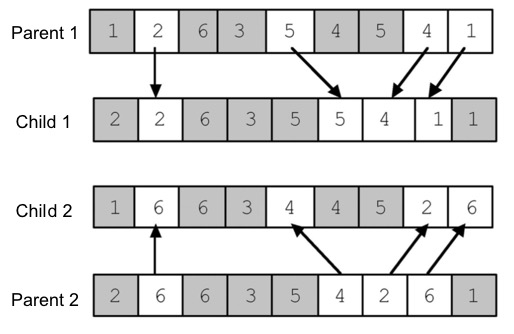
\includegraphics[width=0.6\linewidth]{sections/figure1.jpg}
		\caption{POX crossover operator based on job sequence encoding}
		\label{fig:fig1}
	\end{center}
\end{figure}

\subsection{Selection operartor}
Selection operator decides whether an individual enters the next generation based on its fitness value, which is defined as the objective function.
The selection operator in genetic algorithm uses both strategies of elite model and tournament selection.
The former identifies the best 1\% individuals in the current generation and allows them entering into the next generation directly without crossover.
Tournament selection works by randomly selecting two individuals from the current generation and then chooses the one with better fitness value if a random number $r \in (0,1)$ is smaller than a predefined value $k$ which is set as 0.8. 
Note that the chosen one will be allowed to be selected again in the next iteration of tournament selection.



\subsection{Improved genetic algorithm design}
Traditional genetic algorithm does not perform well in solving scheduling problems due to the acceptance of new offsprings created though the crossover operator, even if their fitness values are worse than that of their parent solutions, during which process good solutions are lost and damaged.
This paper proposes an improved genetic algorithm utilizing a new offspring solution creation strategy.
In this strategy, 2$n$ offspring solutions are created from $n$ iterations of crossover operators applied on two parent solutions, the two best offspring solutions are chosen as the final offspring solutions to enter the next iteration.
Computational results show that the improved algorithm performs superior than traditional genetic algorithm in both convergence rate and solution quality.
For example, the optimal solution with objective value of 930 is obtained using the improved genetic algorithm in solving the famous benchmark instance FT10.
The algorithmic workflow is as follows:
\begin{enumerate}
	\item randomly create $P$ chromosome individual solutions and compute their corresponding objective values.
	\item output the optimal solution if the stopping criteria is met; go to the next stop otherwise.
	\item select the offspring solutions for the next generation according to the selection operator.
	\item (1) apply crossover operator with probability $P_c$ on parent solution $n$ times to create 2$n$ offspring solutions, from which two best solutions are selected as the final offspring solutions; (2) apply mutation probability $P_m$ on offspring solutions to create mutated offsprings.
	\item create new population and return to step 2.
\end{enumerate}
